% ---------------------------------------------------------------------------
% Author guideline and sample document for EG publication using LaTeX2e input
% D.Fellner, v1.20, Jan 18, 2023

\documentclass{egpubl}
\usepackage{eurovis2024}
\usepackage{comment}
\usepackage{amsmath}

% --- for  Annual CONFERENCE
% \ConferenceSubmission   % uncomment for Conference submission
% \ConferencePaper        % uncomment for (final) Conference Paper
% \STAR                   % uncomment for STAR contribution
% \Tutorial               % uncomment for Tutorial contribution
% \ShortPresentation      % uncomment for (final) Short Conference Presentation
% \Areas                  % uncomment for Areas contribution
% \Education              % uncomment for Education contribution
% \Poster                 % uncomment for Poster contribution
% \DC                     % uncomment for Doctoral Consortium
%
% --- for  CGF Journal
% \JournalSubmission    % uncomment for submission to Computer Graphics Forum
% \JournalPaper         % uncomment for final version of Journal Paper
%
% --- for  CGF Journal: special issue
% \SpecialIssueSubmission    % uncomment for submission to , special issue
%\SpecialIssuePaper         % uncomment for final version of Computer Graphics Forum, special issue
%                          % EuroVis, SGP, Rendering, PG
% --- for  EG Workshop Proceedings
% \WsSubmission      % uncomment for submission to EG Workshop
 \WsPaper           % uncomment for final version of EG Workshop contribution
% \WsSubmissionJoint % for joint events, for example ICAT-EGVE
% \WsPaperJoint      % for joint events, for example ICAT-EGVE
% \Expressive        % for SBIM, CAe, NPAR
% \DigitalHeritagePaper
% \PaperL2P          % for events EG only asks for License to Publish

% --- for EuroVis 
% for full papers use \SpecialIssuePaper
% \STAREurovis   % for EuroVis additional material 
% \EuroVisPoster % for EuroVis additional material 
% \EuroVisShort  % for EuroVis additional material
% \MedicalPrize  % uncomment for Medical Prize (Dirk Bartz) contribution, since 2021 part of EuroVis

% Licences: for CGF Journal (EG conf. full papers and STARs, EuroVis conf. full papers and STARs, SR, SGP, PG)
% please choose the correct license
%\CGFStandardLicense
\CGFccby
%\CGFccbync
%\CGFccbyncnd


% !! *please* don't change anything above
% !! unless you REALLY know what you are doing
% ------------------------------------------------------------------------
\usepackage[T1]{fontenc}
\usepackage{dfadobe}  
\usepackage{algorithm}
\usepackage{algpseudocode}
\usepackage{subfigure}
\usepackage{xspace}
\usepackage{booktabs}


\usepackage{cite}  % comment out for biblatex with backend=biber
% ---------------------------
%\biberVersion
\BibtexOrBiblatex
%\usepackage[backend=biber,bibstyle=EG,citestyle=alphabetic,backref=true]{biblatex} 
%\addbibresource{egbibsample.bib}
% ---------------------------  
\electronicVersion
\PrintedOrElectronic
% for including postscript figures
% mind: package option 'draft' will replace PS figure by a filename within a frame
\ifpdf \usepackage[pdftex]{graphicx} \pdfcompresslevel=9
\else \usepackage[dvips]{graphicx} \fi

\usepackage{egweblnk}
\newcommand*{\vtkm}{\mbox{VTK-m}\xspace}
\newcommand{\poincare}{Poincar\'{e}\xspace}

\usepackage{xcolor}

\newcommand\dave[1] {\textcolor{red}{\textbf{Dave: #1}}}

\definecolor{authora}{RGB}{105, 41, 197}
\newcommand*{\ken}[1]{\textcolor{authora}{\textbf{Ken: #1}}}

% end of prologue

\title {Performance Improvements of \poincare\ Analysis for Exascale Fusion Simulations}

% for anonymous conference submission please enter your SUBMISSION ID
% instead of the author's name (and leave the affiliation blank) !!
% for final version: please provide your *own* ORCID in the brackets following \orcid; see https://orcid.org/ for more details.
\author[D. Pugmire et al.]
{\parbox{\textwidth}
{
\centering 
D. Pugmire$^{1}$\orcid{0000-0003-0647-2634},
J. Y. Choi$^{1}$\orcid{0000-0002-6459-6152},
S. Klasky$^{1}$\orcid{0000-0003-3559-5772},
K. Moreland$^{1}$\orcid{0000-0002-7051-3288},
E. Suchyta$^{1}$\orcid{0000-0002-7047-9358},
T. M. Athawale$^{1}$\orcid{0000-0003-3163-6274},
Z. Wang$^{1}$\orcid{0000-0003-1123-9925},
C.-S. Chang$^{2}$\orcid{0000-0002-3346-5731},
S.-H. Ku$^{2}$\orcid{0000-0002-9964-1208}, and
R. Hager$^{2}$\orcid{0000-0002-4624-3150}
}
\\
{\parbox{\textwidth}{
\centering
$^1$Oak Ridge National Laboratory, USA\\
$^2$Princeton Plasma Physics Laboratory, USA
}
}
}

% ------------------------------------------------------------------------

% if the Editors-in-Chief have given you the data, you may uncomment
% the following five lines and insert it here
%
% \volume{36}   % the volume in which the issue will be published;
% \issue{1}     % the issue number of the publication
% \pStartPage{1}      % set starting page

%-------------------------------------------------------------------------
\begin{document}

% uncomment for using teaser
% \teaser{
%  
\includegraphics[width=0.9\linewidth]{eg_new}
%  \centering
%   \caption{New EG Logo}
% \label{fig:teaser}
%}

\maketitle
%-------------------------------------------------------------------------
\begin{abstract}
Understanding the time-varying magnetic field in a fusion device is critical for the successful design and construction of clean-burning fusion power plants. \poincare analysis provides a powerful method for the visualization of magnetic fields in fusion devices. However, \poincare plots can be very computationally expensive making it impractical, for example, to generate these plots in situ during a simulation.
In this short paper, we describe a collaboration among computer science and physics researchers to develop a new \poincare tool that provides a significant reduction in the time to generate analysis results. \\
%Leave one blank line after the abstract, then add the subject categories according to the ACM Classification Index 
%-------------------------------------------------------------------------
%  ACM CCS 1998
%  (see https://www.acm.org/publications/computing-classification-system/1998)
% \begin{classification} % according to https://www.acm.org/publications/computing-classification-system/1998
% \CCScat{Computer Graphics}{I.3.3}{Picture/Image Generation}{Line and curve generation}
% \end{classification}
%-------------------------------------------------------------------------
%  ACM CCS 2012
%   (see https://www.acm.org/publications/class-2012)
%The tool at \url{http://dl.acm.org/ccs.cfm} can be used to generate
% CCS codes.
%Example:
% \begin{CCSXML}
% <ccs2012>
% <concept>
% <concept_id>10010147.10010371.10010352.10010381</concept_id>
% <concept_desc>Computing methodologies~Collision detection</concept_desc>
% <concept_significance>300</concept_significance>
% </concept>
% <concept>
% <concept_id>10010583.10010588.10010559</concept_id>
% <concept_desc>Hardware~Sensors and actuators</concept_desc>
% <concept_significance>300</concept_significance>
% </concept>
% <concept>
% <concept_id>10010583.10010584.10010587</concept_id>
% <concept_desc>Hardware~PCB design and layout</concept_desc>
% <concept_significance>100</concept_significance>
% </concept>
% </ccs2012>
% \end{CCSXML}
%
% \ccsdesc[300]{Computing methodologies~Collision detection}
% \ccsdesc[300]{Hardware~Sensors and actuators}
% \ccsdesc[100]{Hardware~PCB design and layout}
%
\begin{CCSXML}
<ccs2012>
   <concept>
       <concept_id>10003120.10003145.10003147.10010364</concept_id>
       <concept_desc>Human-centered computing~Scientific visualization</concept_desc>
       <concept_significance>500</concept_significance>
       </concept>
   <concept>
       <concept_id>10003120.10003145.10003146</concept_id>
       <concept_desc>Human-centered computing~Visualization techniques</concept_desc>
       <concept_significance>300</concept_significance>
       </concept>
   <concept>
       <concept_id>10010405.10010432.10010441</concept_id>
       <concept_desc>Applied computing~Physics</concept_desc>
       <concept_significance>100</concept_significance>
       </concept>
 </ccs2012>
\end{CCSXML}

\ccsdesc[500]{Human-centered computing~Scientific visualization}
\ccsdesc[300]{Human-centered computing~Visualization techniques}
\ccsdesc[100]{Applied computing~Physics}

\printccsdesc   
\end{abstract}  

\section{Introduction}
\label{sec:intro}

%Due date: Feb 23. Notification: April 10\\
Outline:
\begin{enumerate}
    \item Introduction
    \begin{itemize}
        \item Fusion
        \item Motivation- magnetic fieldline analysis in fusion
        \item Very expensive, want to do much more frequently.
        \item Contributions....
    \end{itemize}
    \item Related work
    \item Methods
    \begin{itemize}
    \item poincare algorithm
    \item mapping this 
    \end{itemize}
    \item Results
    \begin{itemize}
        \item Results from Summit. Number of points, locators, etc.
        \item Results from Frontier. 
    \end{itemize}
    \item Future work
\end{enumerate}

Fusion energy research is focused on understanding the science needed to develop energy sources based on the controlled fusion of light atomic nuclei. Fusion energy is an active area of research that promises to provide large amounts of clean energy.
One promising avenue for achieving fusion energy is using a machine called a tokamak. A tokamak confines a plasma using magnetic fields within a torus.
Scientists around the world are actively researching high-fidelity models to predict the performance and behavior of fusion in tokamak devices. Significant efforts are currently underway to plan experiments on the International Thermonuclear Experimental Reactor (ITER) tokamak under construction in France.
ITER, and follow-on devices, will operate in physics regimes not achieved by any current or past experiments, making advanced and predictive numerical simulation critical for success.


The tokamak contains many magnetic coils producing a strong magnetic field that confines the charged particles within the plasma. One set of magnetic coils generates an intense  \emph{torroidal} field, in the direction around the torus. A second set of coils generates a magnetic \emph{poloidal} field in the direction around a cross-section of the torus. These two fields result in a twisted magnetic field that twists the plasma, resulting in confinement.  Additional coils are used to drive the shape of the plasma during confinement.

The time-varying behavior of the magnetic fields is complex and vital to the performance of the tokamak. This makes analysis tools for understanding the dynamic nature of the magnetic field critical. The complexity of the three-dimensional, periodic magnetic field lines makes direct visualization difficult.
Because the field lines are periodic, the complexity can be reduced by making use of a recurrence or \poincare map. This technique reduces the dimension of each field line from three down to two by intersecting the periodic orbit with a lower-dimensional subspace (called the \poincare section).
Here we intersect each field line with a plane to create a sequence of points. The pattern produced by each field line provides valuable insight into the topology of the complex magnetic field lines inside the plasma.

Proper characterization of the magnetic field requires a large number of orbits to a large number of field lines. It is common to create \poincare maps containing tens of thousands of field lines, each consisting of thousands of orbits.
In practice, the field lines are computed using particle advection to trace the path of massless particles through the magnetic field. Calculating the orbit of each field line consists of taking a large number of advection steps using a numerical solver. To ensure the accuracy of such long field lines, an appropriately small step size must be used for the numerical solver. This in turn results in a large number of solves for each orbit. As an example, for an orbit that takes $500$ advection steps, computing $1000$ orbits results in 500,000 advection steps for each field line. For 50,000 field lines, this results in a total of $2.5 x 10^{10}$ advection steps.

In this short paper, we describe a collaboration among computer science and physics researchers to provide a significant reduction in the time required to perform \poincare analysis on the magnetic fields in plasma simulations using the X-Point Gyrokinetic Code (XGC)~\cite{HAGER2016644} code.  Before the collaboration began, the tool used by the physicists to perform this analysis took up to several hours. Because of this, the amount of analysis that can be performed was very limited. Further, because the magnetic field evolves over the course of the simulation, a detailed analysis of the time-varying evolution was not possible.
This collaboration resulted in a new \poincare tool being developed using \vtkm \cite{moreland2016vtk}, a visualization toolkit that provides portability across CPUs and GPUs.
This new tool was run on four different workloads using both CPUs and GPUs on a modern supercomputer. It achieved time speedups of between $5.8\times$ and $8.9\times$ on the CPU and between $11.4\times$ and $15.4\times$ on the GPU. In addition, because the new \poincare\ tool required fewer resources, the cost of running was significantly lower. The cost savings for the four workloads were between $14.4\times$ and $22.4\times$ for the CPUs and between $58.4\times$ and $77.1\times$ for the GPU.

One of the major challenges in this collaboration was ensuring that the complex representation in the simulation code of the magnetic field was accurately conveyed in the new visualization tool.
The \vtkm accelerated tool has made it possible for \poincare analysis to be performed in situ for large-scale simulations running on supercomputers located at the Oak Ridge Leadership Computing Facility (OLCF)~\cite{Suchyta2022}.

\begin{comment}
acceleration of the 

The fusion scientists with whom we are collaborating had a tool for generating \poincare maps that ran on multi-core CPUs.  Generating \poincare map from a single timestep in a simulation using $50,000$ field lines of $3000$ orbits took about $2.5$ hours. \dave{Lookup the numbers from the summit runs.}
Because of this cost, \poincare map analysis was done infrequently.

The resulting field lines are intersected with the \poincare section to produce the result.








The behavior and evolution of the magnetic fields in a tokamak are complex, and its control is critical for performance making analysis tools for 
Because of this, analysis tools for understanding the dynamic nature of the magnetic field are critical.
The complexity of the three-dimensional magnetic field lines makes analysis and visualization difficult.
Because the field lines are periodic, this complexity can be reduced by using a \poincare magnetic field-line puncture map~\cite{poincare}. 
The \poincare map is the intersection of a field line with a lower-dimensional subspace (called the \poincare section).
In our case, the \poincare section is a two-dimensional plane that is perpendicular to the axis of the tokamak.
Given a set of magnetic field lines, the \poincare map, i.e., intersection of the magnetic field lines with the plane, provides a concise 
representation of the magnetic field that is easier to understand and analyze.
Figure~\ref{fig:poincare} shows some examples of \poincare plots.

In practice, the \poincare map is generated by creating a large number of field lines and plotting each intersection, or puncture, with the plane.
After a sufficient number of punctures have been collected, patterns in the map characterize the features in the magnetic field.
The field lines are computed by modeling massless particles that follow magnetic field lines.
These massless particles can follow magnetic field lines by advecting them in the direction of the magnetic field.
The intersections generated from a single particle characterize the features of the magnetic surface at that position.
The particles are advected using a differential equation solver, such as the 4$^{\text{th}}$ order Runge-Kutta scheme.

In practice, proper characterization of the magnetic field requires a large number of initial positions (typically tens of thousands), each of which typically results in between 1000 and 3000 intersections with each intersection coming from following a field line all the way through the tokamak's torus.
Because of this, the computation of a \poincare map can be very expensive.
The WDMApp team has a \poincare map code that runs on CPUs and takes several hours for the largest analysis runs. 
%Because of this cost, the generation \poincare maps required careful planning.
The high cost of the analysis was due to two main factors. First, the large numbers of particles and intersections required previously mentioned, and second, the complexity of the magnetic field calculation.  In many applications of particle advection, the vector field is calculated at the nodes of each cell in the mesh. Linear interpolation within the cell is used to evaluate the magnetic field for the particle being advected. Because of the large number of advection steps required for each particle in the \poincare map, small errors can rapidly accumulate. These errors are compounded by the fact that the evaluation of the magnetic field requires a complex set of calculations requiring high-order interpolation of several quantities.

Using \vtkm we can significantly accelerate the computation of \poincare maps using the parallelism available on GPUs. Because the trajectory of each particle is completely independent, the task can be parallelized over each particle. Using this approach, a \poincare map can be computed in under $3$ minutes. The wall-clock time for a typical WDMApp simulation step is between $1.5$ and $2$ minutes, which means that \poincare maps can be computed in situ in nearly real-time.
When WDMApp is run, the workflow control system, EFFIS~\cite{Suchyta2022:effis}, allocates an additional 1 to 2 nodes for the \poincare map analysis. As a simulation step completes, EFFIS launches a \poincare analysis task on GPUs in the node in a round-robin fashion. This allows asynchronous analysis to be performed on the additional nodes while the simulation is running. Figure~\ref{fig:poincare} shows \poincare maps from two different timesteps of a simulation run at the OLCF.
Real-time generation of \poincare maps provides the WDMApp team with unprecedented capability for analysis of magnetic fields in fusion simulations.

Please follow the steps outlined in this document very carefully when
submitting your manuscript to Eurographics.

You may as well use the \LaTeX\ source as a template to typeset your own
paper. In this case we encourage you to also read the \LaTeX\ comments
embedded in the document.


\noindent Long captions should be set as in Figure~\ref{fig:ex1} or
Figure~\ref{fig:ex3}.

\begin{figure}[htb]
   % an empty figure just consisting of the caption lines
   \caption{\label{fig:ex1}
     'Empty' figure only to serve as an example of long caption requiring 
     more than one line. It is not typed centered but aligned on both sides.}
\end{figure}

\noindent
Figures which need the full textwidth can be typeset as Figure~\ref{fig:ex3}.



All graphics should be centered.

%%%
%%% Figure 1
%%%
\begin{figure}[htb]
  \centering
  % the following command controls the width of the embedded PS file
  % (relative to the width of the current column)
  
\includegraphics[width=.8\linewidth]{sampleFig}
  % replacing the above command with the one below will explicitly set
  % the bounding box of the PS figure to the rectangle (xl,yl),(xh,yh).
  % It will also prevent LaTeX from reading the PS file to determine
  % the bounding box (i.e., it will speed up the compilation process)
  % 
\includegraphics[width=.95\linewidth, bb=39 696 126 756]{sampleFig}
  %
  \parbox[t]{.9\columnwidth}{\relax
           For all figures please keep in mind that you \textbf{must not}
           use images with transparent background! 
           }
  %
  \caption{\label{fig:firstExample}
           Here is a sample figure.}
\end{figure}


List all bibliographical references in 9-point Times, single-spaced, at the
end of your paper in alphabetical order. When referenced in the text, enclose
the citation index in square brackets, for example~\cite{Lous90}. Where
appropriate, include the name(s) of editors of referenced books.

\end{comment}
\vspace{-.1in}
\section{Related Work}
\label{sec:related}

\subsection{\poincare Maps}
\poincare maps are an important tool developed for the study of dynamical systems. One of the key advantages is that it provides a dimension reduction to study periodic systems~\cite{morrison2000magnetic}. In the case of our fusion example, this reduction is from 3D to 2D.  L{\"o}effelmann et al.~\cite{Loeffelmann-1997-VPM} provide a summary of the usage of \poincare maps for visualization across a variety of application areas and demonstrate their usefulness in flow analysis.
\poincare maps have been applied to fusion in a number of works, including the following~\cite{Sanderson2010, Sanderson2012understanding, Tricoche2011 }.
%Techniques for computing \poincare maps will be discussed in the following section.


\subsection{Streamlines and Particle Advection}

A widely used visualization algorithm for flow fields is a technique called streamlines \cite{VTKTextbook}.
The technique starts with a velocity vector field representing the flow of a fluid at each point in the domain, which is a common output from computational fluid dynamics simulations.
This fluid is visually represented by one or more curves that trace the trajectory of that part of the flow.
This is modeled and computed as a massless particle instantaneously moving with the velocity determined by the field at the particle's position.
The particle is placed at a seed point and then is advected by pushing it by the vector field.
The computation (described in more detail in Section~\ref{sec:method}) solves a differential equation to find the curve that is tangent to the vector field everywhere.

Although these traces of advected particles can be visualized directly as streamlines, they also form the basis of numerous visualization algorithms, some of which require the advection of a great many particles \cite{Hultquist1992,Guo2016}.
Because particle advection is the greatest computational cost of these algorithms, much research has been invested in optimizing this process \cite{Zhang2018, Yenpure2023}.
The work in this paper leverages the particle advection provided by the VTK-m library \cite{moreland2016vtk}.
VTK-m provides a flexible particle advection algorithm that is optimized for a variety of processors \cite{Pugmire2018}.

Technically, a magnetic field is not a flow field; it does not describe the movement of matter.
However, we are interested in extracting magnetic field lines: curves that are tangent to the magnetic field everywhere.
This is the same property a particle advection trajectory has to its velocity field, and thus it is valid to extract these magnetic field lines by treating magnetism as a flow and leveraging the aforementioned particle advection algorithms.
This paper often refers to flowing particles even though that does not match the physical process.
%\vspace{-.15in}
\section{Methods}
\label{sec:method}

\begin{comment}
\begin{itemize}
    \item Computing field lines through the XGC mesh.
    \item Equation for RK4
    \item Describe XGC mesh
    \item Describe the algorithm
    \item Parallelization with \vtkm.
    \item Convenient to use cylindrical coordinates for tracing.
    \item Evaluation of magnetic fields
    \begin{itemize}
        \item XGC grid (2D triangle grid, N planes)
        \item XGC formulation of magnetic fields
    \end{itemize}
\end{itemize}
\end{comment}

Computing the \poincare map consists of two basic steps. First, compute field lines originating from each seed location. Second, intersect the fieldlines with the \poincare section.
Fieldlines, or streamlines, are generated by computing the trajectory of a massless particle through a  vector field. 
This is a classic initial value problem, $\frac{dy}{dt} = f(t,y)$, where $y(t_0) = y_0$. Here, $y_0$ is the (seed) location at time $t_0$, and $f(t,y)$ is the vector field. For streamline computation, a common method for computing the trajectory of the particle ($y(t)$), is using the $4^{th}$ order Runge-Kutta iterative method~\cite{PresTeukVettFlan92}. For a given step size $h > 0$, positions along the trajectory ($y_i)$ can be computed by:
%\vspace{-.1in}
\begin{align}
    y_{n+1} = y_n  + \frac{h}{6} (k_1 + 2k_2 + 2k_3 + k_4)
    \label{eq:RK4}
\end{align}
\vspace{-.1in}
where
%\vspace{-.1in}
\begin{align*}
k_1 &= f(t_n,\quad y_n) \\
k_2 &= f(t_n+\frac{h}{2},\ y_n + h\frac{k_1}{2}) \\
k_3 &= f(t_n+\frac{h}{2},\: y_n + h\frac{k_2}{2}) \\
k_4 &= f(t_n+\frac{h}{2},\; y_n + hk_3)
\end{align*}
\vspace{-.3in}


\begin{figure}[htb]
  \centering
  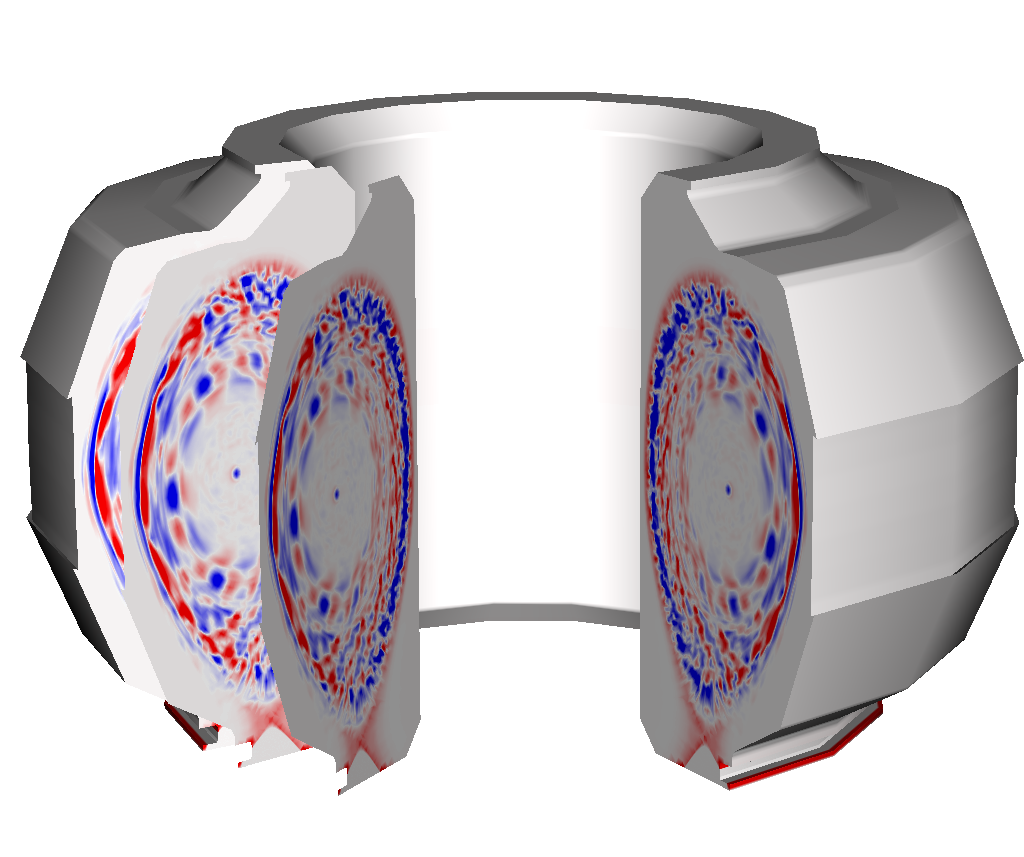
\includegraphics[height=1.5in]{figures/xgc2.png}
\vspace{-.15in}
  \caption{Example of an XGC mesh that has been clipped to show the interior. 2D planes are equally spaced around the central axis of the tokamak. Two planes are shown in the clipped region to illustrate the semi-unstructured nature of the mesh.}
  \label{fig:xgc_mesh}
\end{figure}

The key requirement of the RK4 method is to be able to evaluate $f(t,y)$ (i.e., the magnetic field) at each point within the domain.

The XGC code uses a semi-unstructured mesh to represent the physics of the plasma. Fundamentally, the mesh is cylindrical with periodic boundary conditions along the cylinder's axis. The mesh is structured along the axis of the cylinder and each toroidal cross-section is a 2D unstructured triangular mesh.
The cross-section is rotated around the central axis to create the 3D mesh (see  Figure~\ref{fig:xgc_mesh}).
The mesh consists of wedge elements that are formed from pairs of triangles from adjacent planar cross sections.


\subsection{\poincare Algorithm}
\label{sec:algorithm}
\algnewcommand\algorithmicforeach{\textbf{for each:}}
\algnewcommand\ForEach{\item[ \algorithmicforeach]}

\begin{algorithm}
\caption{Algorithm for computing a \poincare map.}
\label{alg:poinc}

\begin{algorithmic}[1]
\State \textbf{/* Initialization */}
\State $P$ = \poincare section \label{alg:poinc:init0}
\State $S$ = Input seed locations
\State $Max_p$ = Maximum number of punctures
\State $Result = Empty$ \label{alg:poinc:init1}
\State 
\ForAll{$s$ in $S$} \label{alg:poinc:forLoop0}
  \State \textbf{/* Compute the \poincare map for the field line at $s$ */}
  \State $n = 0$ %\bf{ /* Number of punctures for seed */}
  \State $p_0 = s$ 
  \State
  \State \textbf{/* Iterate until max number of punctures computed */}
  \While{$n < Max_p$}  \label{alg:poinc:whileLoop0}
    \State $p_1 = $ RK4Solve($p_0$)
    \State $L = $ line segment from $p_0$ to $p_1$
    \If{$L$ intersects $P$} \label{alg:poinc:intersect_check}
      \State Add intersection of $L$ and $P$ to $Result$
      \State $n = n + 1$
     \EndIf
    \State $p_0 = p_1$
   \EndWhile  \label{alg:poinc:whileLoop1}
\EndFor   \label{alg:poinc:forLoop1}

\end{algorithmic}
\end{algorithm}


Algorithm~\ref{alg:poinc} contains pseudocode for computing the \poincare map.
Initialization consists of specifying the initial seed locations, defining the \poincare section (i.e., 2D plane), and the maximum number of punctures to compute as well as initializing a structure to store punctures (Lines \ref{alg:poinc:init0} - \ref{alg:poinc:init1}).
For each seed location $s$ (Line~\ref{alg:poinc:forLoop0}), the fieldline is iteratively computed using a RK4 solver. At each iteration of the solver, the line segment between the current location and the previous location is checked against the \poincare section to determine if an intersection occurred (Line~\ref{alg:poinc:intersect_check}).
If so, the intersection point is added to the result.
This process continues until the maximum number of punctures occurs, or the particle terminates. For brevity, the code to check for particle termination is not shown in the code listing.

\subsection{Implementation in \vtkm}
\vtkm uses a data parallel abstraction to achieve high performance on many-core devices~\cite{MCD3:2021}.
Given a vector of data, \vtkm will apply a function to each element of the array. These functions often come in the form of ``functors,'' which is an object that can be called like an ordinary function. 
The input data to the \vtkm implementation of the \poincare algorithm is an array of initial particle positions. 
The functor object is initialized with the \poincare section, RK4 step size and the maximum number of punctures.
The execution portion of the functor consists of lines~\ref{alg:poinc:forLoop0}-~\ref{alg:poinc:forLoop1} in Algorithm~\ref{alg:poinc}.
At runtime, each input particle and the functor are mapped to a thread and executed on the specified device, effectively making the for loop parallel.

\begin{comment}
\begin{figure}[htb]
  \centering
  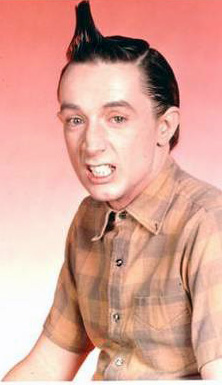
\includegraphics[height=1in]{figures/Ed}
  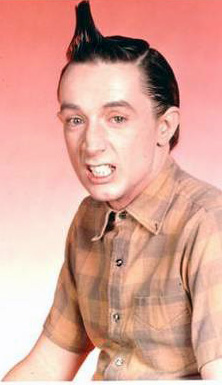
\includegraphics[height=1in]{figures/Ed}

  \caption{Projection of $(x,y,\phi$) onto 2D. Consider tossing this figure.}
  \label{fig:project2d}
\end{figure}
\end{comment}

The bottleneck of the algorithm is not the arithmetic used to compute Equation~\ref{eq:RK4} for the RK4 solution but rather the field evaluation to get the numbers to plug into the equation.
At each iteration of the algorithm, the cell containing the current location of the point must be determined. Because the mesh is unstructured, this requires a cell search. This search can be optimized by taking advantage of the toroidal symmetry of the mesh.
Using this symmetry, the point can be specified by $(x,y,\phi)$, where $x$ and $y$ are coordinates of the 2D cross-section and $\phi$ is the angle around the torus. The point can be easily projected onto the 2D cross section by setting $\phi = 0$ (i.e., $(x,y,0)$).
The cell-finding operation is now reduced to two dimensions.

To accelerate the cell-finding operation for unstructured grids, \vtkm provides two different acceleration structures. The first uses two levels of structured grids~\cite{Kalojanov2011}. The first level is a coarse grid of bins that covers the spatial extents of the data. Each bin within the first level contains a finer grid where the number of bins is proportional to the number of cells contained in the first level grid. Each bin in the fine-level grids contains a list of unstructured cells that are contained.
The second acceleration structure is much simpler. It uses a single fine-structured grid. As before, each bin contains a list of the unstructured cells that are contained.
For each method, the 2D cross-section mesh is passed in, and the acceleration structure is built. The acceleration structure is passed into the \vtkm functor to be used for field evaluations.

The major costs for either structure are the time to retrieve the appropriate bin and the time to search through the cells in the bin.
The advantage of the simpler uniform bin approach is that the appropriate bin can be found with a single lookup rather than the two-part lookup of the two-level grid.
However, the two-level grid avoids bins containing large numbers of unstructured cells when the unstructured cells are unevenly distributed.

In either case, whenever the algorithm looks up a cell, it remembers both the unstructured cell found and the bin containing it.
Subsequent field evaluations will be nearby and are often in the same cell or a nearby one.
Before searching for a bin, the algorithm first checks the saved unstructured cell for containment and then the saved bin.

\subsection{Field Evaluation}
For many applications, the vector field values are defined at the vertices of each cell. Evaluation at a location within the cell interpolates the values at each of the vertices. However, the magnetic field in XGC is much more complicated. Because calculating fieldlines contains many iterative steps, accuracy is paramount as small errors can rapidly grow and produce incorrect results.

In XGC, the magnetic field vector consists of an axisymmetric (i.e., defined at the cross-sectional plane and constant along the cylindrical axis) background field, $\boldsymbol{B}_0$ and a non-axisymmetric perturbation, $\delta\boldsymbol{B}$.
For a particle located at $(x,y,\phi)$, the magnetic field is sum of the background field and the perturbation: $\boldsymbol_{B}_0(x,y) + \delta\boldsymbol{B}(x,y,\phi)$.
The background field, $\boldsymbol{B}_0$,  is evaluated using cubic spline interpolation using the $2D$ coordinates $(x,y)$.
The perturbation is represented as the component of the magnetic vector potential parallel to the background magnetic field $A_\parallel(x,y,\varphi)$, on a set of $N_\varphi$ planar, unstructured triangle meshes, where $N_\varphi$ is the toroidal resolution of the XGC simulation.  In practice, for large runs, $N_\varphi$ is between 32 and 64, depending on the physics being studied. The corresponding perturbed magnetic field is $\delta\boldsymbol{B}=\nabla\times(A_\parallel \boldsymbol{B}_0/|\boldsymbol{B}_0|)$.
For interpolation of data between planes, the magnetic vector potential and its derivatives are interpolated linearly along the magnetic field line through the position of the particle. This requires interpolation on two cross-sectional planes, which is also linear. To minimize interpolation errors, the mesh in XGC is approximately aligned with the magnetic field such that a field line starting on a vertex on one plane maps along $\boldsymbol{B}_0$ to a position at or very close to a mesh vertex on the adjacent plane. For a more detailed explanation is given in~\cite{moritaka_2019, Hariri2013, HAGER2016644}.

Accurately calculating the non-axisymmetric perturbation of the magnetic field, ($\delta\boldsymbol{B}$), was the most challenging part of the collaboration.
The XGC implementation of the \poincare\ tool is embedded within the XGC simulation code. The \poincare\ tool is run by using an input deck for the simulation that specifies how to configure and run the analysis. As such, the code for performing a full simulation and \poincare\ analysis share some non-trivial overlap that must be carefully separated. Further, given that XGC is written in Fortran, and \vtkm is written in C++, the code separation must be done carefully and is easy to get wrong. We instrumented the XGC code with debug logs to check the calculation of key quantities in the derivation of the magnetic field at each step of a point along a field line. The coordinates of individual field lines were also saved so that they could be compared (both visually and textually) to the coordinates generated by the \vtkm implementation. When differences in coordinates were detected, we were able to compare, step by step, the computation of the different values associated with the calculation of $\boldsymbol{B}_0$ and $\delta\boldsymbol{B}$ in both codes and determine where the errors occurred. Once these were identified and fixed, we ran both the XGC and \vtkm implementations of the code over many different seeding scenarios and physics parameters and compared the resulting \poincare plots to ensure they were identical.

In an attempt to optimize the calculation of the perturbed magnet field, we pre-computed $\boldsymbol_{B}_0(x,y) + \delta\boldsymbol{B}(x,y,\phi)$ at each vertex in the $3D$ mesh to avoid the complexity of the field evaluation at every RK4 iteration. However, the effects of linear interpolation of the values within the 3D elements of the mesh over a large number of iterations resulted in errors that compounded over thousands of RK4 steps and produced significantly inaccurate results. In the end, this optimization had to be abandoned.


\begin{comment}
\begin{itemize}
  \item Magnetic field vector consists of an axisymmetric (i.e., constant in the cylindrical angle $\varphi$) background and a non-axisymmetric perturbation
  \item The background field $\boldsymbol{B}_0$ is fully described by two functions, $\psi(R,Z)$, where $R$ and $Z$ are cylindrical coordinates, and $F(\psi)$. (Can add the formula, if necessary.)
  \item The background field is evaluated using cubic spline interpolation using only the marker position $(R,Z)$.
  \item The perturbation is represented as the component of the magnetic vector potential parallel to the background magnetic field, $A_\parallel(R,Z,\varphi)$, on a set of $N_\varphi$ planar, unstructured triangle meshes, where $N_\varphi$ is the toroidal resolution of the XGC simulation. 
  \item The corresponding perturbed magnetic field is $\delta\boldsymbol{B}=\nabla\times(A_\parallel \boldsymbol{B}_0/|\boldsymbol{B}_0|$.
  \item For interpolation of data between planes, the magnetic vector potential and its derivatives are interpolated linearly along the magnetic field line through the position of a marker. This requires interpolation on two $(R,Z)$ planes, which is also linear.
  \item To minimize interpolation errors, the mesh in XGC is approximately aligned with the magnetic field such that a field line starting on a vertex on one plane maps along $\boldsymbol{B}_0$ to a position at or very close to a mesh vertex on the adjacent plane.
  
\end{itemize}
\end{comment}
 








\section{Results}
\label{sec:results}

The experiments were performed on the Frontier~\cite{frontier} supercomputer at Oak Ridge National Laboratory.
%Summit is a 200 PetaFLOPS supercomputer that consists of 4608 nodes. Each node contains two 22-core IBM Power9 CPUs and six NVIDIA Tesla V100 GPUs.
Frontier is a 1.102 ExaFLOPS supercomputer consisting of 9472 nodes. Each node contains a 64-core AMD Epyc CPU and four Radeon Instinct MI250X GPUs. 


\begin{comment}
\begin{figure}[ht]
 \centering
  \subfigure[Whole seeding]{
    \label{fig:seedingUniform}  
     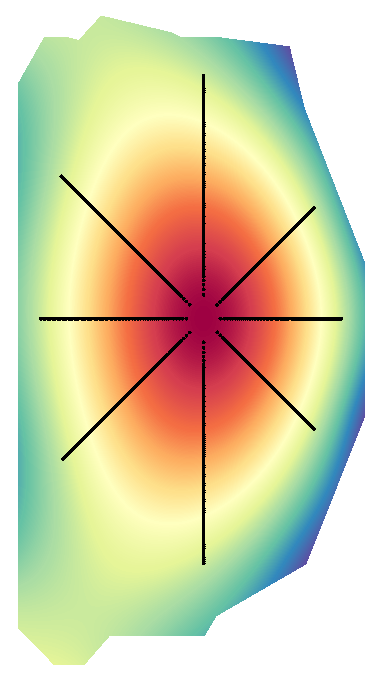
\includegraphics[width=25mm]{figures/seedingWhole}
   }
  \subfigure[Edge seeding]{
   \label{fig:seedingEdge}  
   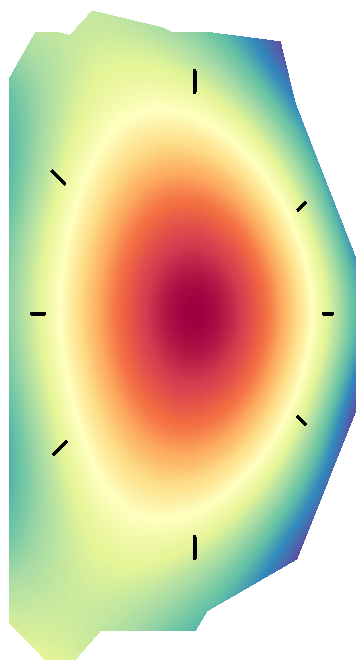
\includegraphics[width=25mm]{figures/seedingEdge}
   }

\caption{Seed placement provides opportunities for analysis of different parts of the plasma. Whole seeding (a), provides an overall view of the magnetic field. Edge seeding (b), is useful to analyze the outer region of the plasma where turbulence is very high. }
\vspace{-5pt}
\label{fig:seeding}
\end{figure}
\end{comment}


\begin{figure}[ht]
 \centering
  \subfigure[Whole seeding]{
    \label{fig:seedingUniform}  
     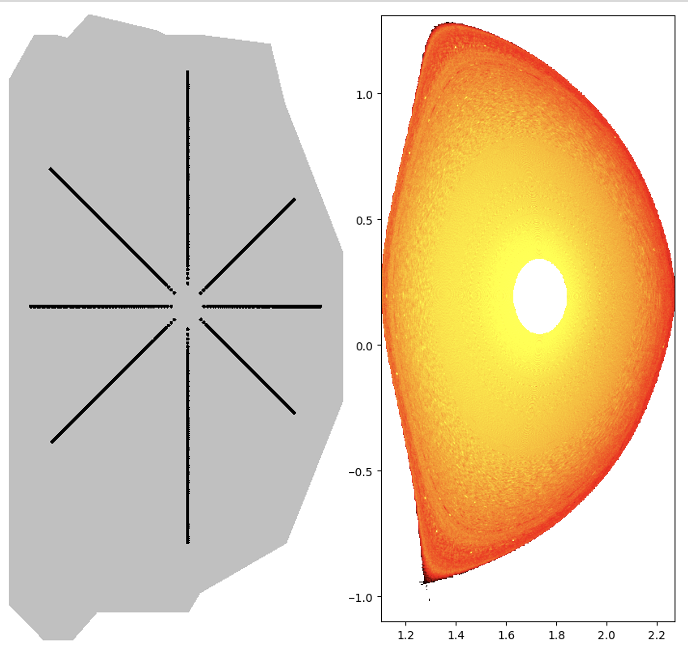
\includegraphics[height=30mm]{figures/wholeSeedingAndResult}
   }
  \subfigure[Edge seeding]{
   \label{fig:seedingEdge}  
   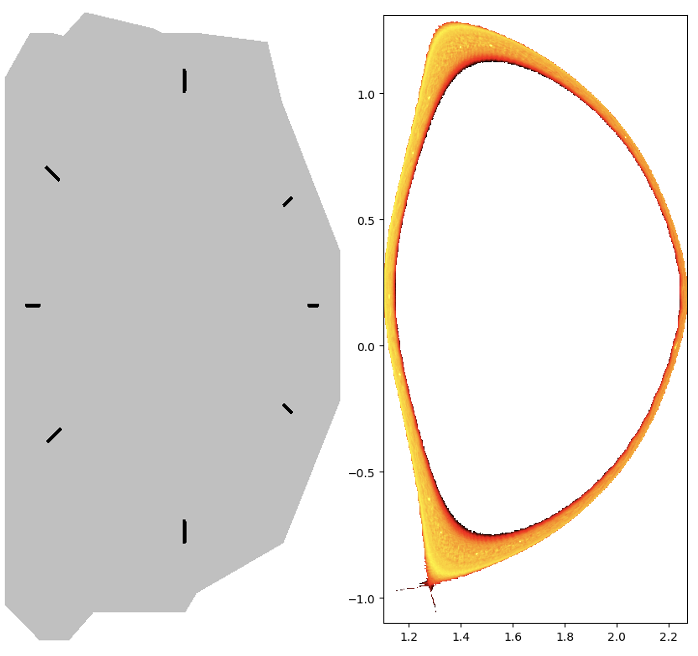
\includegraphics[height=30mm]{figures/edgeSeedingAndResult}
   }

\caption{Seed placement allows for analysis of different parts of the plasma. Whole seeding along with the resulting \poincare map is shown in (a), and the edge seeding and results are shown in (b).}
\vspace{-5pt}
\label{fig:seeding}
\end{figure}


To study the performance, we ran both the XGC and \vtkm versions of the \poincare tool. We use the XGC implementation as a baseline. While the XGC simulation code can run on GPUs, the XGC \poincare\ analysis tool is only implemented on the CPUs. 
The \vtkm implementation was run on both the CPU and GPU. The results from the runs on CPUs give us a direct comparison between the XGC analysis code and the \vtkm equivalent. The runs on the GPU highlight the added benefits afforded by the portability of the \vtkm implementation.

The XGC implementation was run on the CPUs of five Frontier nodes and uses OpenMP for parallelization across the multi-core CPUs.
The \vtkm implementation was run in two configurations -- CPU and GPU.
The CPU implementation was run on two Frontier nodes and the GPU implementation was run on a single node using two of the four GPUs.

We used two variations in the number of seeds and two variations in the placement of the seeds for a total of four different configurations.
The seeds are placed along regular angular intervals around the center of the cross-section. We used a total of eight angular intervals and placed $1280$ and $3200$ seeds along each angular interval. This gives seed numbers of 10,240 and 25,600. We also varied the placement of the seeds along each angular interval. For whole seeding (see Figure~\ref{fig:seedingUniform}), the seeds are placed uniformly from the center of the cross-section to the edge. For edge seeding (see Figure~\ref{fig:seedingEdge}), the seeds are placed further away from the center, or nearer to the edge of the plasma.  Whole seed placement is used to analyze the overall nature of the magnetic field in the plasma. The placement of seeds along the edge is a common way to analyze the very turbulent regions of the plasma that occur along the edge region. Figure~\ref{fig:result} shows a zoomed-in view of \poincare maps generated from two different time steps using edge seeding. The image is zoomed in to view the bottom left of the cross-section, called the ''X'' point, where turbulence in the plasma is complex.


\begin{comment}
\begin{figure}[ht]
 \centering
  \subfigure[Whole seeding. ]{
    \label{fig:resultUniform}  
     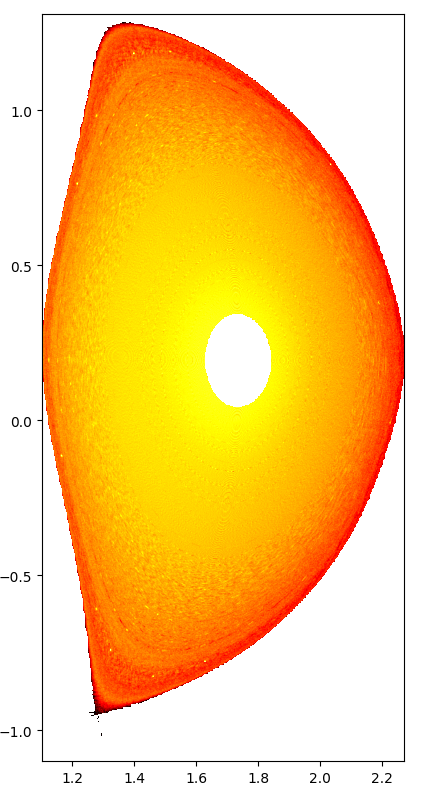
\includegraphics[width=20mm]{figures/whole}
     }
  \subfigure[Edge seeding.]{
   \label{fig:resultEdge}  
   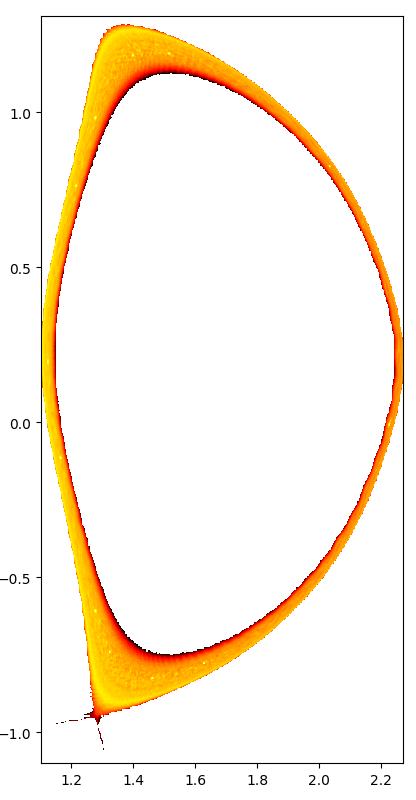
\includegraphics[width=20mm]{figures/edge}
   }

\caption{Resulting \poincare plots from 10,240 seeds using whole (a) and edge (b) seeding.}
\vspace{-5pt}
\label{fig:result}
\end{figure}
\end{comment}


\begin{figure}[ht]
 \centering
 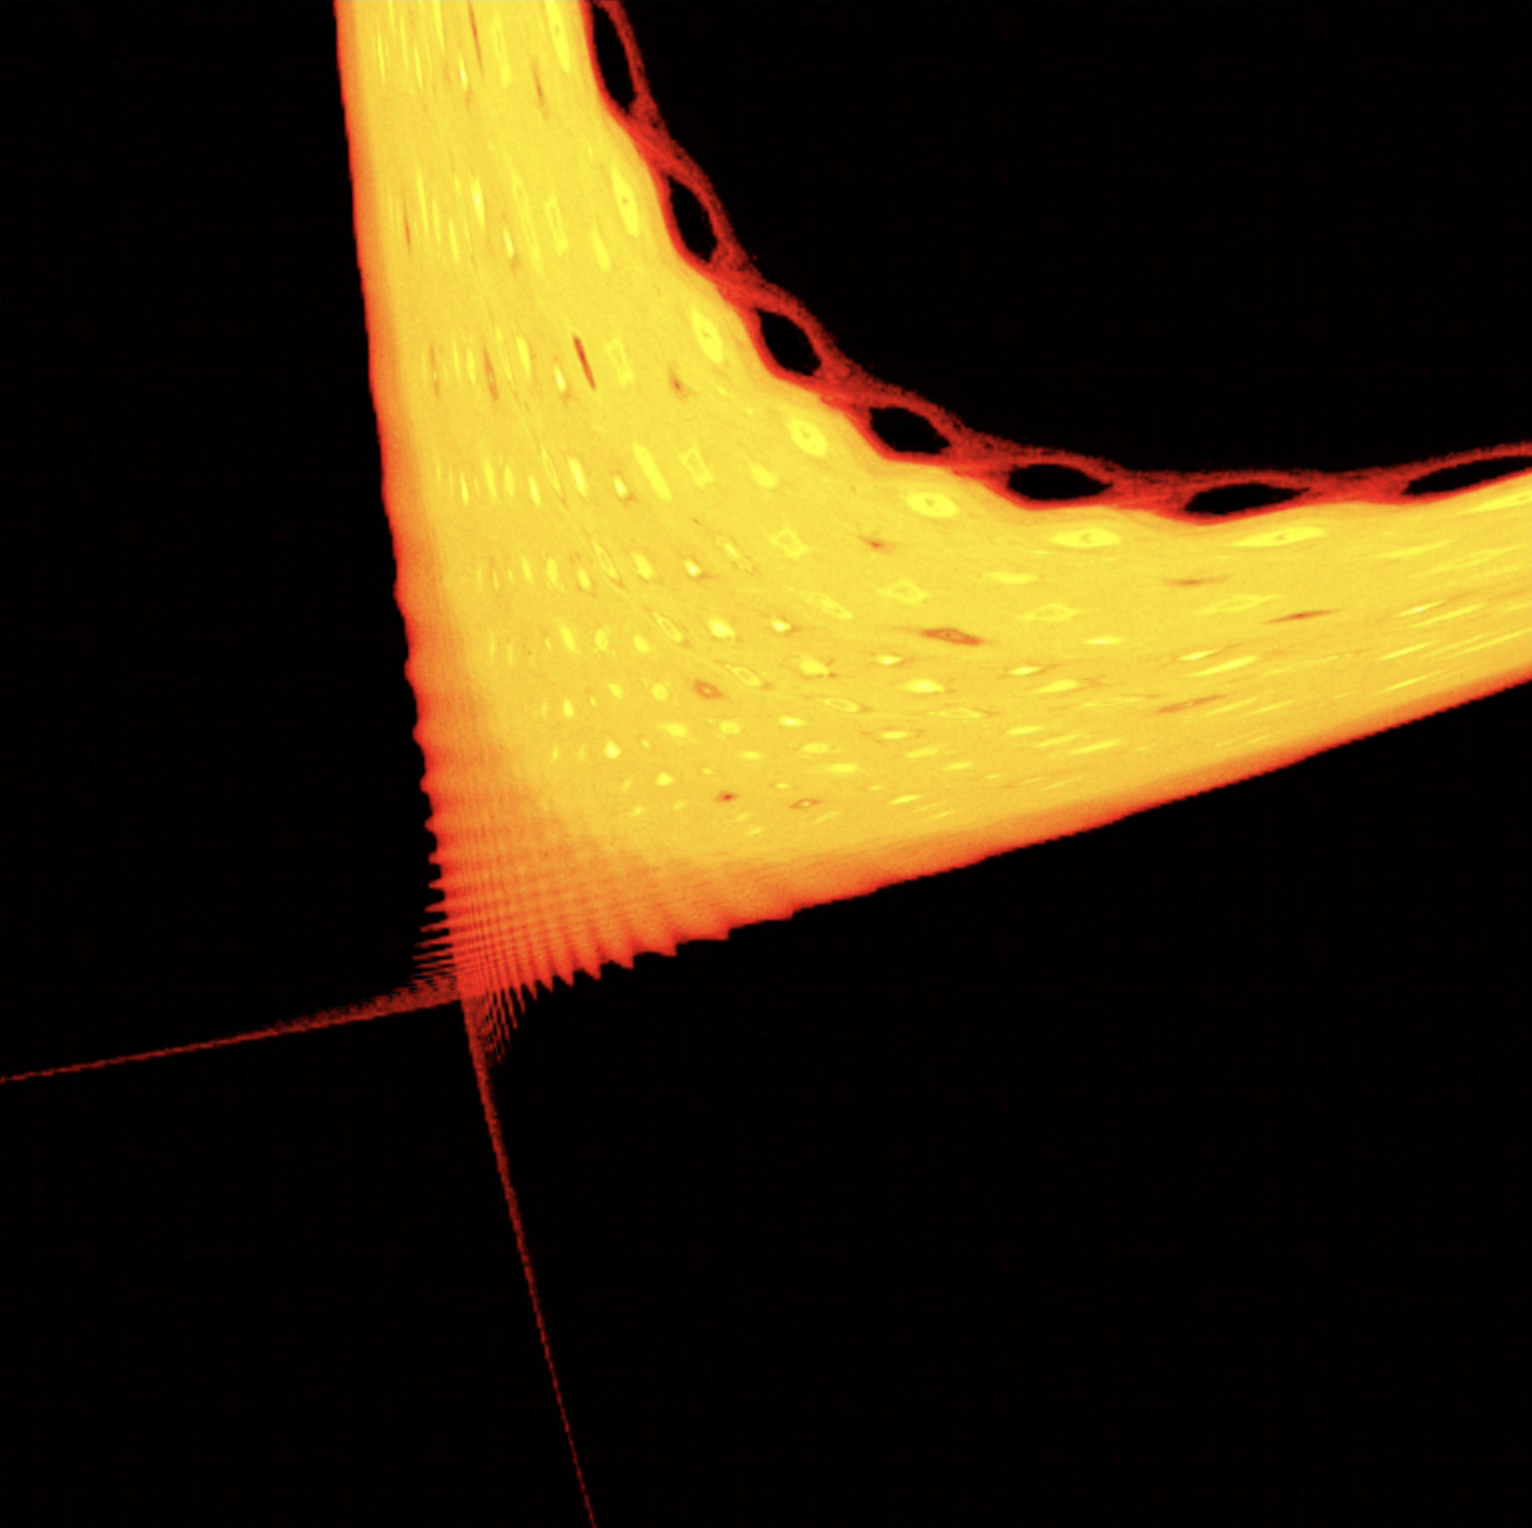
\includegraphics[width=40mm]{figures/poincare-X.1.png}
 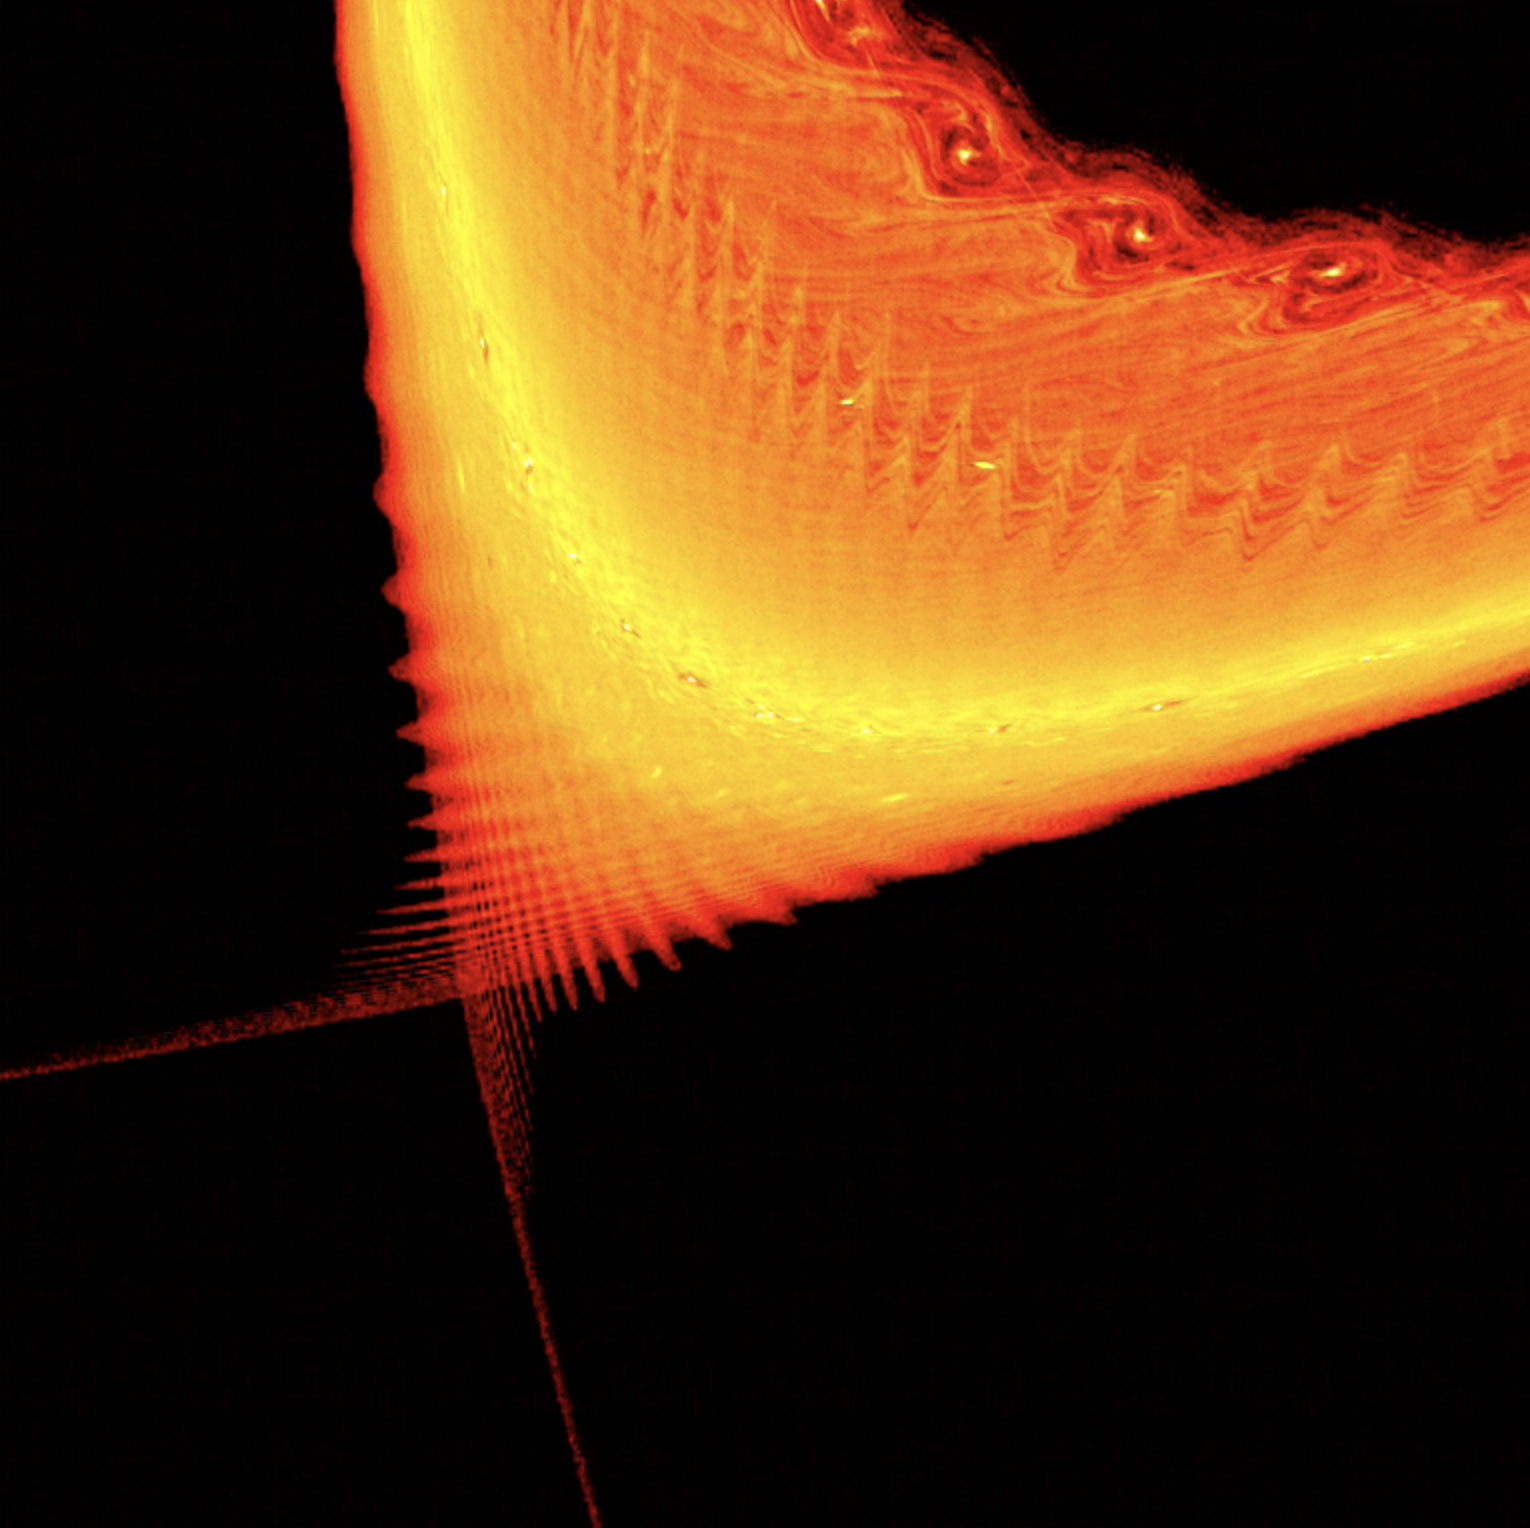
\includegraphics[width=40mm]{figures/poincare-X.2.png}

\caption{\poincare maps generated from two time steps using edge seeding. Zooming in to regions of interest makes it possible to see topological features that develop as the plasma develops.}
\vspace{-5pt}
\label{fig:result}
\end{figure}








\begin{table}[]
\centering
\caption{Time (in seconds) for XGC and \vtkm runs on CPUs and GPUs for both Whole and Edge seeding with $10,240$ and $25,600$ seeds. The time speedup factors for the \vtkm runs on the CPU and GPU are given in two right-most columns.}
\label{table:timingResults}
\begin{tabular}{ll|c|cc|cc}
\hline
\textbf{Num} & \multicolumn{1}{c|}{} & \textbf{XGC} & \multicolumn{2}{c|}{\textbf{VTK-m Time}} & \multicolumn{2}{c}{\textbf{Speedup}} \\
\textbf{Seeds} & \textbf{Seeding} & \textbf{Time} & \textbf{CPU} & \textbf{GPU} & \textbf{CPU} & \textbf{GPU} \\ \hline \hline
10240 & Whole & 2001.8 & 249.0 & 171.5 & \textbf{8.0} & \textbf{11.7} \\
10240 & Edge & 1762.6 & 197.0 & 154.3 & \textbf{8.9} & \textbf{11.4} \\
25600 & Whole & 3785.8 & 655.5 & 245.7 & \textbf{5.8} & \textbf{15.4} \\
25600 & Edge & 3435.3 & 522.0 & 223.1 & \textbf{6.6} & \textbf{15.4} \\ \hline
\end{tabular}
\end{table}


Table~\ref{table:timingResults} contains the timing results for the XGC tool and \vtkm implementations for each configuration.
We also ran the \vtkm implementations using both the Two-Level and Uniform Bins cell locators, but the performances were similar (within $1.5\%$ of each other). The results we report are using the Uniform Bins cell locator. Because the triangles in the cross-sectional grid are uniformly distributed, the added complexity of the Two-Level grid does not provide any benefit. We performed some tuning on the optimal size of the Uniform Bin acceleration structure and found that a size of 12,000$\times$12,000 generally provided the best results.
The speedups for the \vtkm implementation are significant. Running on the CPU, the \vtkm implementation provides between $5.8\times$ and $8.9\times$ speedup over the XGC implementation. On the GPU, \vtkm achieves between $11.4\times$ and $15.4\times$ speedup over the XGC implementation. 
Speedups on the GPU are limited by two factors. First, the number of threads that can be utilized. The computation is parallelized over the seeds, and the number of seeds commonly used for \poincare maps is not enough to saturate the number of threads available on the GPUs. Second, and much more importantly, the cell-finding operation for unstructured grids is bound by the cost of memory access and \emph{not} computation. As the seeds are traced, they circulate throughout the volume in non-uniform ways. Because the acceleration structure used for cell-finding is too large to be kept in fast GPU memory, there is significant time spent accessing data in slower memory spaces.

%\ken{A reviewer might why we don't have a chart for the data in table 1 and/or table 2.}


Table~\ref{table:costSavings} contains a comparison of the total cost (in node-seconds) for the XGC and \vtkm implementations for each configuration. The XGC tool was run on five nodes of Frontier and so the XGC Cost column in Table~\ref{table:costSavings} is $5\times$ the runtime reported in Table~\ref{table:timingResults}. For the \vtkm implementation, the CPU runs were performed on two nodes of Frontier, and the GPU runs were performed on two GPUs within a single node.  Because of this difference in the number of nodes used, the cost savings for the \vtkm implementation are more pronounced than the speedups. For the CPU runs, the \vtkm implementation running on two nodes, results in cost savings between $14.4\times$ and $22.4\times$. For the GPU runs, the \vtkm implementation results in cost savings between $57.1\times$ and $77.1\times$.  We calculate the cost factor for \vtkm using one node, although it technically uses only half of the node, which results in cost savings between $114.2\times$ and $154.2\times$.

The use of fewer nodes becomes even more important when doing in situ processing. XGC uses the in-transit processing model~\cite{ChildsTerminology, Choi2018} for in situ analysis and visualization tasks. In this model, additional nodes are allocated for analysis and visualization. After the simulation completes a time step, the data are transferred to the additional nodes for asynchronous processing.
For simulations that could run for days or weeks, the use of fewer nodes for analysis and visualization results in even more significant cost savings.




\begin{comment}
\begin{table}[]
\caption{Time (in seconds) for XGC and \vtkm runs using the Two-Level (2L) and Uniform Bins (UB) cell locators. The speedup (SU) over the XGC runs is also given for each cell locator type.}
\label{table:timingResults}
\centering
\begin{tabular}{@{~}r@{~~}crr@{~~}rr@{~~}r@{~}}
  \toprule
      &                              & \multicolumn{1}{c}{XGC}      & \multicolumn{2}{c}{\vtkm 2L}                 & \multicolumn{2}{c}{\vtkm UB} \\
  \multicolumn{1}{c@{~~}}{\# Seeds} &
  \multicolumn{1}{@{~~}c}{Seeding} &
  \multicolumn{1}{c}{Time} &
  \multicolumn{1}{c@{~~}}{Time} &
  \multicolumn{1}{@{~~}c}{SU} &
  \multicolumn{1}{c@{~~}}{Time} &
  \multicolumn{1}{@{~~}c}{SU} \\
  \midrule
10240 & Whole & 2001.83 & 168.45 & \textbf{11.88} & 171.49    & \textbf{11.67}   \\
10240 & Edge    & 1762.64 & 150.71 & \textbf{11.70} & 154.29    & \textbf{11.42}   \\
25600 & Whole & 3785.81 & 258.51 & \textbf{14.64} & 245.66    & \textbf{15.41}   \\
25600 & Edge    & 3435.26 & 229.30 & \textbf{14.98} & 223.08    & \textbf{15.40}   \\
  \bottomrule
\end{tabular}
\end{table}
\end{comment}

\begin{table}[]
\centering
\caption{Total cost (in node-seconds) for XGC and the savings factor for the \vtkm runs on the CPU and GPU.
The XGC runs used five nodes and the \vtkm used two Frontier nodes for the CPU runs and one node for the GPU runs.
%\textcolor{red}{Jay: should the metric here be core-time and the unit is node-seconds?} and savings factor for \vtkm.
}
\label{table:costSavings}
\begin{tabular}{ll|r|rr}
\hline
\textbf{Num} & \multicolumn{1}{c|}{} & \multicolumn{1}{c|}{\textbf{XGC}} & \multicolumn{2}{c}{\textbf{VTK-m Cost Savings}} \\
\textbf{Seeds} & \textbf{Seeding} & \multicolumn{1}{c|}{\textbf{Cost}} & \textbf{CPU} & \textbf{GPU} \\ \hline \hline
10240 & Whole & 10009.2 & \textbf{20.1} & \textbf{58.4} \\
10240 & Edge & 8813.2 & \textbf{22.4} & \textbf{57.1} \\
25600 & Whole & 18929.1 & \textbf{14.4} & \textbf{77.1} \\
25600 & Edge & 17176.3 & \textbf{16.5} & \textbf{77.0} \\ \hline
\end{tabular}
\end{table}


\begin{comment}
\begin{table}[]
\caption{Total cost (in node-seconds) for XGC and the savings factor (Factor) for the \vtkm runs using both cell locators.
The XGC runs used five nodes and the \vtkm runs used one Frontier node.
%\textcolor{red}{Jay: should the metric here be core-time and the unit is node-seconds?} and savings factor for \vtkm.
}
\label{table:costSavings}
\centering
\begin{tabular}{r@{~~}crrr}
\toprule
\multicolumn{1}{l}{}          &                              & \multicolumn{1}{c}{XGC}           & \multicolumn{1}{c}{\vtkm 2L} & \multicolumn{1}{c}{\vtkm UB} \\
\multicolumn{1}{c@{~~}}{\# Seeds} & \multicolumn{1}{@{~~}c}{Seeding} & \multicolumn{1}{c}{Cost} & \multicolumn{1}{c}{Factor}   & \multicolumn{1}{c}{Factor}   \\ 
\midrule
10240 & Whole & 10009.15 & 59.42 & 58.37 \\
10240 & Edge    & 8813.20   & 58.48 & 57.12 \\
25600 & Whole & 18929.05 & 73.22 & 77.05 \\
25600 & Edge    & 17176.30  & 74.91 & 77.00 \\
\bottomrule
\end{tabular}
\end{table}
\end{comment}








\begin{comment}
Results on frontier. Kokkos setting:
1000x10 pts, 10 puncs, UB 12000 12000

Setting hints from none, 2 to 1024
0: PoincareTime= 4.59509239
2: PoincareTime= 8.996044041
4: PoincareTime= 5.383845941
8: PoincareTime= 3.334134504
16: PoincareTime= 2.443431037
32: PoincareTime= 1.830533336
64: PoincareTime= 2.019787151
128: PoincareTime= 2.086194197
256: PoincareTime= 2.109982273
512: PoincareTime= 4.521679962
1024: PoincareTime= 6.577413594

1000x10 pts, 100 puncs
0: PoincareTime= 44.886269575
2: PoincareTime= 86.530851057
4: PoincareTime= 53.34156569
8: PoincareTime= 31.379374444
16: PoincareTime= 22.082198616
32: PoincareTime= 15.638019499
64: PoincareTime= 18.477414351
128: PoincareTime= 18.550843151
256: PoincareTime= 20.639840234
512: PoincareTime= 45.01590981
1024: PoincareTime= 76.879381214

Hints=32
whole:
10k x 1000: 149.154060158
25k x 1000:  309.024710581
edge: 
10k x 1000: 140.758010554
25k x 1000: 


whole: 10k x 1000
Hints-32  149.154060158
Hints=64  180.872969537
Hints=128  187.471073264

whole: 25k x 1000
Hints=32 309.024710581
Hints=64 267.215708676
Hints=128 267.135570261


Vary UB:
10k x 10punc
12: 1.811252
10: 1.665629376
8: 1.548936766
4:  1.443947304
2: 1.527570323
but at 100 puncs, 10k 12k is best.


10k x 1000punc, UB12
Whole
H32: 147.828542898
H64: 182.412161965
H128: 187.174267512

Edge
H32: 139.308568648
H64: 154.220764795
H128: 155.587906359

25k x 1000punc, UB12
Whole
H32: 309.551289458
H64: 269.644134008
H128: 267.333313573

Edge
H32: 290.064207587
H64: 223.823065319
H128: 221.518910766



2L:
8 2 1.422736871
16 2 1.398853571
32 2 1.972269867
64 2 2.044388573
128 2 2.075921773


openmp

\end{comment}

\section{Summary and Future Work}
\label{sec:conclusion}
In this paper, we have described a collaborative effort among computer scientists and physicists to develop a new tool for performing analysis and visualization of the magnetic fields in fusion devices. \poincare\ plots are notoriously expensive to generate due to high computational costs. Because of the complexity of the magnetic fields in tokamaks, the definition of the vector field needed for generating field lines is often code-specific and complex. Working together with the XGC physics team, we developed a tool that reproduces the complex definition of the magnetic field and uses the concepts in \vtkm to efficiently map the computation onto both multi-core CPU and GPU devices.  The development of this new tool has made it possible for physicists to perform unprecedented analysis on XGC simulations running on some of the most powerful supercomputers in the world. Previously, it was only possible to perform \poincare\ analysis on a limited number of timesteps from a simulation. This work has made it possible to generate \poincare\ plots in situ for every time step of the simulation. This provides the XGC team with a powerful new tool to study the physics of burning plasmas.

Although we have achieved significant speedups in computing \poincare maps, there is still room for additional performance. The bottleneck in the algorithm is the cost of cell location. There are two major ways to address this problem. The first is to avoid performing cell locations using an adaptive step-sized solver. These techniques improve over the brute-force nature of fixed step-size methods to adjust according to the local changes in the vector field. We plan to explore the use of these solvers to increase performance while maintaining accuracy.
The second is to improve the performance of the cell location on GPUs. The costs for memory access can vary dramatically on the GPU depending on where the memory is located. We plan to explore methods to achieve better caching of data in faster memory to improve overall performance.

%\ken{One thing that I think is missing from this paper is at least one image of a \poincare plot that shows its utility. Figure \ref{fig:result} has results, but they are boring. Can we change this to conclusions and show a picture with a \poincare plot with interesting features? Maybe homoclinic tangles. Maybe just islands.}


\section*{Acknowledgements}

This research used resources of the Oak Ridge Leadership Computing Facility, which is a DOE Office of Science User Facility supported under Contract DE-AC05-00OR22725.
This work was supported in part by the U.S. Department of Energy (DOE) RAPIDS SciDAC project under contract number DE-AC05-00OR22725 and by the Exascale Computing Project (17-SC-20-SC), a collaborative effort of the U.S. Department of Energy Office of Science and the National Nuclear Security Administration.


%-------------------------------------------------------------------------
% bibtex
\bibliographystyle{eg-alpha-doi} 
\bibliography{references}       

% biblatex with biber
% \printbibliography                

\end{document}

